\setcounter{chapter}{-1}

\newchapter{Логика и множества (факультативно)}

Данная глава носит справочный характер и может быть пропущена при первом чтении конспекта. Тем не менее, настоятельно рекомендуется регулярно возвращаться к ней по мере освоения материала.


\section{Суждения и силлогизмы}

\subsection{Конспект}
\begin{enumerate}\setlength{\itemsep}{1pt}
\item Типовая конструкция суждения: \textbf{Посылки} $\vdash$ \textbf{Вывод}.
\item Пример:

\begin{tabular}{lr}
\begin{minipage}[b]{0.6\linewidth}
(\textit{Все птицы --- животные}) и (\textit{все воробьи --- птицы}),

вывод: (\textit{все воробьи --- животные}).

Такой вывод является правильным независимо от того, правильные ли посылки.

(\textit{Все птицы --- животные}) и (\textit{все цветы --- птицы}), вывод: (\textit{все цветы --- животные}).

Это суждение истинно независимо от ложности посылок. Суждение показывает \textit{только взаимосвязь} посылок и вывода. Принцип <<чушь на входе --- чушь на выходе>>.
\end{minipage}&  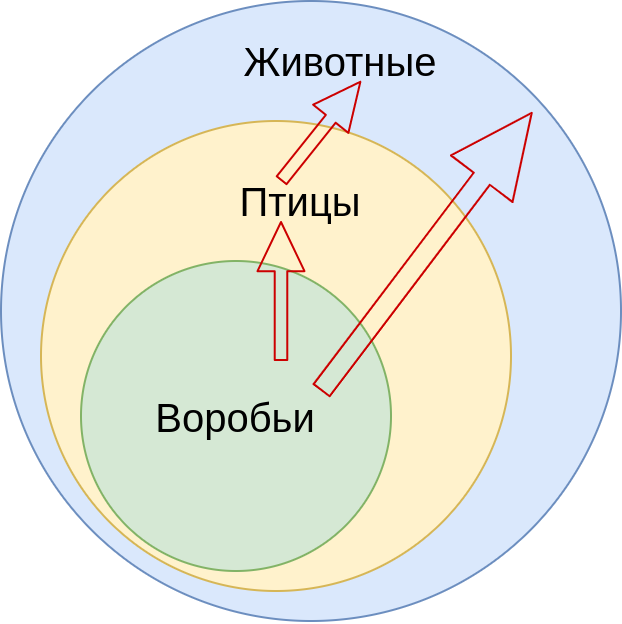
\includegraphics[scale=0.2]{piaf.png}
\end{tabular}
\item При построении суждения посылки могут быть ложными. Более того, в математической логике из ложной посылки следует все, что угодно. Например, \textit{если снег черный, то лес зеленый}. Лес при этом может быть зеленым (летом) и не быть таковым (зимой), но суждение остается истинным, т.к. посылка про снег является ложной.
\item Сравните: если запись числа $a$ оканчивается на 0, то оно кратно 5. Здесь мы ничего не знаем про число $a$, но если для него выполняется посылка, то выполняется и вывод. А если не выполняется, то истинность самого сужджения при этом никак не страдает. Более того, мы знаем, что на 5 также делятся и другие числа, и это значит, что путать местами посылки и вывод ни в коем случае нельзя! Ведь \textbf{не всегда верно}, что если число делится на 5, то его запись заканчивается на 0.
\item Другой~пример:\nopagebreak

\begin{tabular}{lr}
\begin{minipage}[b]{0.5\linewidth}
(\textit{Некоторые французы --- блондины}) и (\textit{некоторые ученики --- французы}), следовательно, (\textit{некоторые ученики --- блондины}). \textbf{Такое суждение неверно}. Поскольку слово <<некоторые>> не гарантирует, что таковым признаком обладают все французы. А значит, из свойства <<быть французом>> не всегда следует <<быть блондином>>.
\end{minipage}& 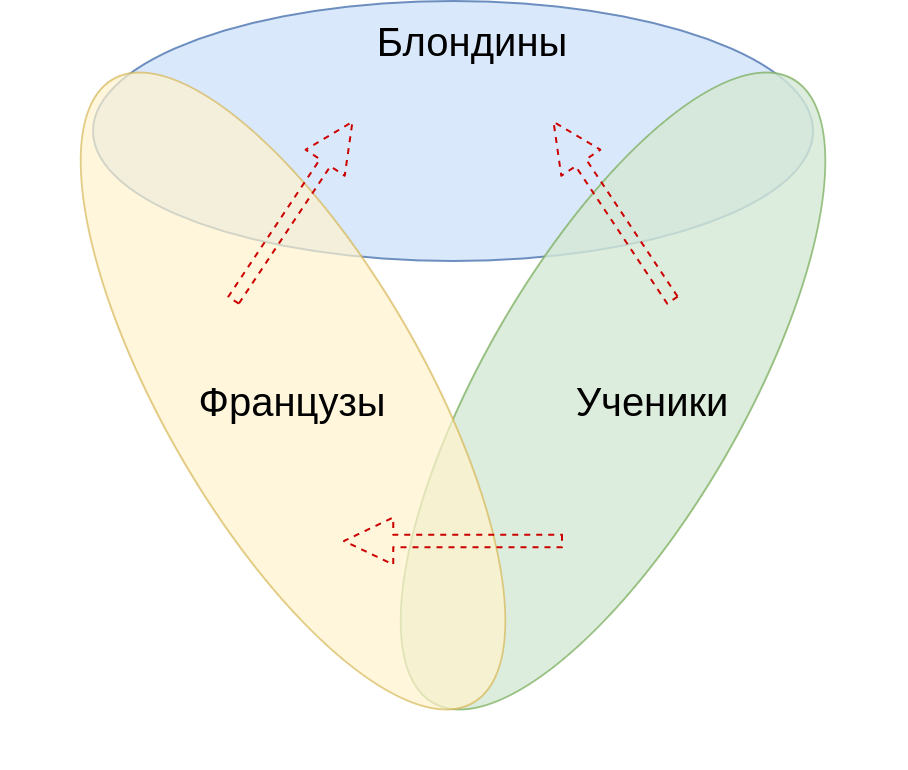
\includegraphics[scale=0.19]{some.png}
\end{tabular}
\item Здесь обе посылки истинные, но вывод ложный. Хотя легко представить ситуацию, когда некоторые ученики действительно будут блондинами. Но это --- лишь предположение, а не строгое рассуждение.
\item В этом примере нарушается именно связка между посылками и выводом, т.к. две посылки не склеиваются по общему признаку. В первой посылке стоит <<некоторые французы>>, а во второй просто <<французы>>, это разные \textbf{множества}, а потому связать две посылки вместе мы не можем!
\item Для построения \textbf{силлогизма} принципиально, чтобы связующее звено было одинаковым:

\begin{center}
\textbf{если} ($A$ есть $B$) и ($B$ есть $C$), \textbf{то} ($A$ есть $C$)
\end{center}
здесь связывание посылок происходит по свойству $B$, и если в нем допустить какое-то искажение, то можно придти к неверным выводам!
\end{enumerate}
\subsection{Задачи}

\section{Высказывания и предикаты}

\subsection{Конспект}
\begin{enumerate}\setlength{\itemsep}{1pt}
\item \textbf{Высказывание} --- это любое утверждение на любом языке, которое может быть либо только истинным, либо только ложным.
\item Примеры высказываний: <<\textit{Шесть больше трех}>>, <<\textit{Дважды два --- пять}>>, <<$\sqrt 2$ --- \textit{число иррациональное}>>, <<\textit{среди натуральных чисел существует наибольшее}>>, <<\textit{всякое четное число является суммой двух простых чисел}>>.
\item Все эти высказывания имеют либо истинное, либо ложное значение, хотя про последнее мы не знаем точный ответ. Но мы точно знаем, что их значения не могут быть переменными, т.е. зависеть от каких-то внешних факторов или других высказываний.
\item Из выше приведенных примеров: <<\textit{все птицы --- животные}>> и <<\textit{все воробьи --- птицы}>> есть истинные высказывания.
\item Но эти высказывания можно разобрать на составляющие. Для чего нам понадобятся предикаты.
\item \textbf{Предикат} --- это суждение, зависящее от переменных, обозначающих объекты данного суждения.
\item Например, <<$x$ \textit{есть воробей}>>, <<$x$ \textit{есть птица}>>, <<$x$ \textit{есть животное}>>. Каждое из них может быть истииным или ложным, смотря что подставить вместо $x$. При $x=$ <<\textit{рыба}>> первые два будут ложными, а при $x=$ <<\textit{ромашка}>> ложными будут все три предиката.
\item Аналогично, <<$x$ \textit{есть ученик}>>, <<$x$ \textit{есть француз}>>, <<$x$ \textit{есть блондин}>>. Заметим, что если ранее мы оперировали \textbf{свойствами} (быть учеником, французом, блондином), то теперь перешли к оперированию \textbf{объектом} $x$, который может обладать тем или иным свойством.
\item Из предикатов можно построить новые предикаты, используя логические связки: И($\land$), ИЛИ($\lor$), НЕ($\neg$), СЛЕДУЕТ($\to$).
\item Например, <<($x$ \textit{есть воробей})$\to$($x$ \textit{есть птица}>>), <<($x$ \textit{есть птица})$\to$($x$ \textit{есть животное}>>). Эти предикаты содержат переменную $x$, но они всегда истинны. Такие тождественно истинные предикаты называются \textbf{тавтологиями}. Тавтологии отличаются от истинных высказываний тем, что содержат переменные, которые можно считать фиктивными. Чтобы тавтологию сделать высказыванием, достаточно перед ним сказать <<\textit{для любого} $x$>>, тогда $x$ перестанет быть параметром, а выражение превратится в истинное высказывание:

\begin{center}
<<(\textit{для любого} $x$) ($x$ \textit{есть воробей})$\to$($x$ \textit{есть птица})>>
\end{center}
\item Это называется правилом введения \textbf{квантора всеобщности}.
\item Далее, рассмотрим высказывание <<\textit{некоторые французы блондины}>>. Поступить аналогично предыдущему и заменить его на  предикат <<($x$ \textit{есть француз})$\to$($x$ \textit{есть блондин})>> нельзя! Дело в том, что высказывание <<\textit{все воробьи --- птицы}>> говорит о вложении одного свойства в другое: быть воробьем означает также быть птицей. Но при слове <<\textit{некоторые}>> мы понимаем, что речь идет не о свойстве <<\textit{быть французом}>>, а о том, что некоторые из французов обладают свойством <<\textit{быть блондином}>>. То есть, мы утверждаем, что существует хотя бы один такой объект $x$, который есть и француз и блондин одновременно!
\item Иначе говоря, мы имеем дело со связкой И:
\begin{center}
($x$ \textit{есть француз})$\land$($x$ \textit{есть блондин}),
\end{center}
данный предикат не всегда является истиной, его истинность зависит от конкретного $x$.
\item Тем не менее, и такой предикат можно превратить в высказывание, причем истинное. Для этого нужно слово <<некоторые>> превратить в <<\textit{существует} $x$>>, так что получится истинное высказывание
\begin{center}
<<(\textit{существует} $x$) ($x$ \textit{есть француз})$\land$($x$ \textit{есть блондин})>>
\end{center}
\item Это называется правилом введения \textbf{квантора существования}.
\item Примеры перевода высказываний с языка свойств на язык объектов:\hfill\;

\begin{tabular}{p{0.4\linewidth}p{0.5\linewidth}}\hline
\textit{Все птицы --- животные}  & (\textit{для любого} $x$) ($x$ \textit{есть птица})$\to$($x$ \textit{есть животное}) \\\hline
\textit{Все воробьи --- птицы}  & (\textit{для любого} $x$) ($x$ \textit{есть воробей})$\to$($x$ \textit{есть птица}) \\\hline
\textit{Все воробьи --- животные}  & (\textit{для любого} $x$) ($x$ \textit{есть воробей})$\to$($x$ \textit{есть животное}) \\\hline
Если число заканчивается на 0, то оно кратно 5 &
(\textit{для любого} $a$) ($a$ \textit{заканчивается на $0$})$\to$($a$ \textit{кратно $5$}) \\\hline
Некоторые французы --- блондины 
& (\textit{существует} $x$) ($x$ \textit{есть француз})$\land$($x$ \textit{есть блондин}) \\\hline
Некоторые ученики --- французы 
& (\textit{существует} $x$) ($x$ \textit{есть ученик})$\land$($x$ \textit{есть француз}) \\\hline
Некоторые ученики --- блондины 
& (\textit{существует} $x$) ($x$ \textit{есть ученик})$\land$($x$ \textit{есть блондин}) \\\hline
\end{tabular}

\item Видим, что построить вывод можно только в том случае, когда две посылки склеиваются по общему предикату <<$x$\textit{ есть птица}>>, при этом сами посылки являются импликациями (следование).
\item Можно комбинировать общие и частные суждения:
\begin{center}
<<($x$ \textit{есть птица})$\land$(\textit{все птицы --- животные})>>,
\end{center}
откуда следует вывод <<($x$ \textit{есть животное})>>.

Здесь мы объединили в посылке предикат, что-то говорящий о свойстве объекта $x$, с высказыванием, которое что-то говорит о связи двух свойств, и нашли новое свойство объекта $x$. Это типичное рассуждение от общего к частному.
\item Построение выводов из заданных или полученных ранее истинных высказываний и предикатов называется \textbf{дедукцией} и является основным методом рассуждений при получении математических теорем.
\item Иногда для построения нужного вывода требуетя перебрать сотни комбинаций ранее доказанных посылок. Но часто для нащупывания правильной цепочки доказательства хватает вспомогательных иллюстраций или опыта исследователя, погруженного в данную тему.
\item Ранее мы отмечали, что рассуждения в обратную сторону --- от вывода к посылкам --- неверны. Однако очень часто это верно отчасти. Например, мы знаем дедуктивный вывод: если число оканчивается на 0, то оно делится на 5. На основе этого мы не можем доказать точно, но \textbf{можем предположить}, что если число делится на 5, то оно, вероятно, может оканчиваться на 0. Как мы знаем, это верно примерно в половине случаев. Если бы такое \textit{разворачивание импликации} было бы всегда абсолютно невозможным, то дедукция представляла бы собой простейший случай вывода, когда ложь влечет любое суждение. Для построения теорий это абсолютно бесполезно.
\item Метод \textit{рассуждения назад}, к уже известной посылке, называется \textbf{абдукцией}. Именно таким методом, как правило, пользовался Шерлок Холмс в своих умозаключениях. Именно поэтому его выводы всегда носят вероятностный характер и сопровождаются словами <<вероятно>>, <<скорее всего>> и т.п. Искусство Шерлока Холмса заключается в том, чтобы из всех возможных посылок в данной конкретной ситуации выбрать наиболее вероятную.
\item Например, цитируем из рассказа <<Этюд в багровых тонах>> (Конан Дойль),

\textit{<<Этот человек по типу --- врач, но выправка у него военная. Значит, военный врач. Он только что приехал из тропиков --- лицо у него смуглое, но это не природный оттенок его кожи, так как запястья у него гораздо белее. Лицо изможденное, --- очевидно, немало натерпелся и перенес болезнь. Был ранен в левую руку --- держит ее неподвижно и немножко неестественно. Где же под тропиками военный врач-англичанин мог натерпеться лишений и получить рану? Конечно же, в Афганистане>>. Весь ход мыслей не занял и секунды. И вот я сказал, что вы приехали из Афганистана.}

\item Рассмотрим только часть умозаключений Холмса и сравним их с арифметическим примером\hfill\;

\begin{tabular}{p{0.55\linewidth}p{0.4\linewidth}}\hline
Ватсон --- военный врач с изможденным лицом и загорелый & 
Число 30 --- делится на 5 \\
Воевавшие в Афганистане --- военные с изможденным лицом и загорелые &
Оканчивающее на 0 число --- делится на 5 \\\hline

Вывод: Ватсон прибыл из Афганистана & Вывод: 30 оканчивается на 0\\\hline
\end{tabular}

\item Как видим, нам дано две посылки, в одной из которых дается некая связь между свойствами (воевашие есть военные и т.д., а также оканчивающиеся на 0 делятся на 5), а в другой дается свойство конкретного объекта (Ватсон и число 30). Это свойство общее в обеих посылках, но по нему нельзя склеить их в силлогизм, т.к. свойство всегда стоит в конце посылки. Но Холмс знает, что практически все военные с изможденным лицом и загорелые --- это воевашие в Афганистане (хотя это и неверно на 100\%), и на основании этого он предполагает(!), что и Ватсон такой же, раз он обладает таким же свойством.

\item На примере числа 30 это тоже сработало, однако стоит нам подставить 25 вместо 30, как вся цепочка рассуждений порушится! Поэтому абдуктивные умозаключения нельзя считать математическими, однако они могут навести на правильное дедуктивное умозаключение, в результате чего либо появляется теорема (\textit{Все военные с изможденным лицом воеали в Афганистане}), либо обнаруживается контрпример (в нашем случае это число 25, которое опровергает предположение о том, что все делящиеся на 5 числа оканчаиваются на 0).
\end{enumerate}

\subsection{Задачи}



\section{Связь предикатов и множеств}

\subsection{Конспект}
\begin{enumerate}
\item Выше мы оперировали такими понятиями как свойство и объект, обладающий свойством, на основе чего вводили различные высказывания и предикаты. Посмотрим, как они связаны с понятием \textbf{множество}.
\item Пусть $M$ --- множество всех людей, живущих на планете. Тогда предикат $h(x)$ <<$x$ есть человек>> можно переписать следующим способом: $h(x)=(x\in M)$. Это одновременно означает и то, что $x$ находится в множестве $M$, и то, что $x$ обладает свойством <<быть человеком>>. Говорят также, что $M$ есть область истинности предиката $h(x)$. Таким образом, множество олицетворяет собой свойство, а элементы множества --- объекты, обладающие данным свойством.
\item Если множество $X$ является частью множества $Y$, (например, множество всех женщин есть часть множества $M$), то мы пишем $X\subseteq Y$ ($X$ \textit{содержится в} $Y$, $Y$ \textit{включает} $X$). Важно не путать значки $\in$ и $\subseteq$, т.к. первй говорит о принадлежности объекта к свойству, а второй --- о вложении свойств (о том, что одно свойство меньше или равно другому). Используется также символ строгого вложения $\subset$, означающий, что вложение имеется, но при этом множества не равны.
\item Вложение множеств выражается с помощью принадлежности:
$$
X\subseteq Y\mbox{ эквивалентно }(\forall x) (x\in X)\to(x\in Y)
$$
По сути, это ровно то же самое, что мы ранее делали при переводе языка свойств на язык объектов: \textit{все $X$ есть $Y$} равносильно высказыванию (\textit{для любого} $x$) ($x$ \textit{обладает свойством} $X$)$\to$($x$ \textit{обладает свойством} $Y$).
\item Обозначим далее: $p(x)$ предикат <<$x$ \textit{есть воробей}>>, $o(x)$ предикат <<$x$ \textit{есть птица}>>, $a(x)$ предикат <<$x$ \textit{есть животное}>>. Ранее мы получали следующий вывод:
$$
(\forall x) (p(x)\to o(x))\land (\forall x) (o(x)\to a(x))\vdash(\forall x) (p(x)\to a(x))
$$
\item Попробуем то же самое выразить множествами. Обозначим через $P$ область истинности предиката $p(x)$, т.е. множество всех воробьев, $O$ --- множество всех птиц, $A$ --- множество всех животных. Тогда написанный выше с помощью предикатов вывод можно записать на языке множеств так:
$$
(P\subseteq O\subseteq A) \vdash (P\subseteq A),
$$
поскольку все воробьи есть птицы, все птицы есть животные, а в итоге все воробьи есть животные.
\item На самом деле, существует намного более тесная связь между логическими связками и операциями над множествами.
Вернемся снова к картинке про французов, блондинов и учеников. На ней есть три множества, обозначенные соответствующими овалами. Обозначим их следующим способом:
$$
F = \{x\mid x\mbox{ --- француз}\},\quad B = \{x\mid x\mbox{ --- блондин}\},\quad E = \{x\mid x\mbox{ --- ученик}\}
$$
\item Здесь можно увидеть примеры \textbf{пересечений} множеств:
\begin{gather*}
F\cap B = \{x\mid (x\mbox{ --- француз})\land (x\mbox{ --- блондин})\},\\
F\cap E = \{x\mid (x\mbox{ --- француз})\land (x\mbox{ --- ученик})\},\\
E\cap B = \{x\mid (x\mbox{ --- ученик})\land (x\mbox{ --- блондин})\}.
\end{gather*}
Видим, что они соответствуют логической связке И соответствующих предикатов, выражающих свойства.
\item На той же схеме мы можем усмотреть и такие теоретико-множественные конструкции, как:
$$
F\setminus B = \{x\mid (x\mbox{ --- француз})\land \neg(x\mbox{ --- блондин})\},
$$
т.е. множество французов, не являющихся блондинами. $F\setminus B$ есть операция \textbf{вычитания} множеств.
\item Наконец, множество 
$$
F\cup E  = \{x\mid (x\mbox{ --- француз})\lor (x\mbox{ --- ученик})\}
$$
представляет собой свойство быть французом ИЛИ учеником. Оно содержит в себе как всех французов, так и всех учеников, причем среди них есть как французы, не являющиеся учениками, так и французы, являющиеся уничениками, а также ученики, не являющиеся французами. \textbf{Объединение} множеств соответствует логической связке ИЛИ.
\item Итак, мы можем легко оперировать предикатами, представляя, что они выражают свойство объекта принадлежать некоторому множеству, и наоборот, оперировать множествами, представляя, что оперируем предикатами, для которых эти множества суть область истинности. При этом И соответствует пересечению, ИЛИ --- обединению множеств. Отрицание соответствует вычитанию множеств, причем разность $X\setminus Y$ можно рассматривать как пересечение $X\cap(\neg Y)$. Наконец, вложение множеств соответствует импликации предикатов.
\end{enumerate}



\subsection{Задачи}
\begin{enumerate}
\item Выразить свойство <<\textit{быть учеником и блондином одновременно}>> через множества $E$ и $B$.
\item Написать множество, соответствующее всем <<\textit{птицам, не являющимся воробьями}>> через множества $O$ и $P$.
\item Какие элементы содержит множество $P\setminus A$, множество $M\cap F$, множество $(F\cup B)\setminus (F\cap B)$?
\item Что выражает высказывание $(M\setminus F)\subseteq (M\setminus B)$?
\item Докажите: $(E\subseteq F)\vdash (M\setminus F)\subseteq (M\setminus E)$ (от противного).
\end{enumerate}


\section{Построение множеств}


\section{Парадоксы}





\newchapter{Визуальная арифметика}

%\renewcommand{\sectionname}{Тема}

\section{Сложение и вычитание}

\subsection{Конспект}
\begin{enumerate}\setlength{\itemsep}{1pt}
\item Берем произвольную прямую, и на ней будем откладывать отрезки --- вправо и влево.
\item Откладывание вправо есть прибавление длины, а откладывание влево --- вычитание (уменьшение) длины.
\item Можно откладывать ноль, т.е. ничего не делать. В этом случае все равно --- прибавляем или вычитаем ноль.
\item Мы можем комбинировать откладывание отрезков вправо и влево, т.е. производить серию последовательных откладываний отрезков (они могут быть разными по длине), на каждом шаге --- от текущей точки положения.
\item Результат \textit{серии откладываний} равносилен одному откладыванию отрезка, соединяющего стартовую и финишную точки, причем финишная точка:
\begin{itemize}
\item может быть справа от стартовой (результатом является одно откладывание вправо, т.е. прибавление длины),
\item может совпадать с ней (результатом оказалось нулевое откладывание)
\item или быть слева от стартовой точки (результатом является одно откладывание влево, т.е. вычитание).
\end{itemize}
\item Откладывание \textit{изотропно}, т.е. одинаковые серии откладываний, приложенные к разным стартовым точкам, приводят к одинаковым результирующим отрезкам, отложенным от этих стартовых точек. Иначе говоря, величина и направление откладывания не зависит от начального местоположения!
\end{enumerate}
\begin{tabular}{ll}
\begin{minipage}{0.6\linewidth}
\begin{enumerate}\setlength{\itemsep}{1pt}\setcounter{enumi}{6}
\item Серии откладываний можно проиллюстрировать складным метром. Раскладывание колена на $180^o$ означает прибавление его длины к общей серии откладываний, а складывание --- вычитание его длины из общей серии откладываний. При этом от стартовой точки можно уйти как вправо, так и влево, или остаться на месте.
\end{enumerate}
\end{minipage}
&
\begin{minipage}{0.4\linewidth}
%\begin{figure}[h]%[htb!]
%\vspace*{3mm}
%\begin{center}
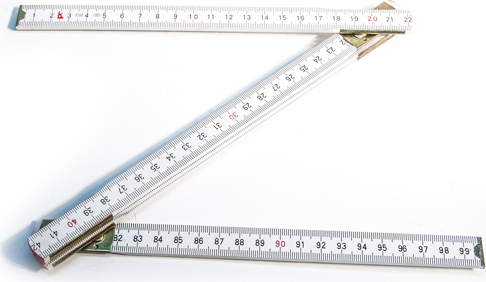
\includegraphics[scale=0.3]{meter.png}
%\end{center}
%\label{meter}
%\end{figure}
\end{minipage}
\end{tabular}
\begin{enumerate}\setlength{\itemsep}{1pt}\setcounter{enumi}{7}
\item С помощью этой же линейки нетрудно продемонстрировать, что композиция откладываний \textbf{ассоциативна} и \textbf{коммутативна}: можно сначала сложить/разложить одну линейку, затем вторую, затем приложить вторую к первой или первую ко второй --- результат будет один и тот же!
\item Кроме того, очевидно, что у каждого откладывания существует обратное, приводящее в результате к нулевому откладыванию. Для этого нужно произвести ровно ту же самую серию откладываний, только поменять ось направления. Или, что то же самое. пройтиь по линейке в обратную сторону.
\item Далее любое откладывание будем записывать буквами $a,b,c,\dots$, имея ввиду под ними как прибавления, так и вычитания.
\item Откладывание, противоположное $a$, будем обозначать $-a$. При этом комбинация откладываний соединяется знаком '+', а если встречается комбинация $a+(-b)$, то пишем проще: $a-b$.
\item Обратные откладывания --- это просто перевернутые в обратную сторону <<линейки>>!
\item Результат откладывания (конфигурацию линейки с учтом ее направления) будем называть \textbf{вектором}. Если вектор смотрит влево (финишная точка левее стартовой), то вектор называется \textit{отрицательным}, а если вправо --- \textit{положительным}. Нулевой вектор --- когда финиш и старт совпадают.
\item Композицию откладываний будем называть \textbf{суммой векторов} или просто суммой, а процедуру откладывания --- \textbf{сложением}.
\end{enumerate}

\textbf{Свойства сложения}:
\begin{enumerate}[SUM1]
\item $(a+b)+c=a+(b+c)$ (ассоциативность);
\item $a+b=b+a$ (коммутативность);
\item $a+0=0+a=a$ (аддитивное свойство нуля);
\item $a+(-a)=0$ (обратный элемент);
\item если $a+x=b+x$, то $a=b$ (правило сокращения);
\item верно одно и только одно: либо $a=b$, либо $a=b+x$, либо $a=b-x$, где $x$ --- откладывание вправо (трихотомия)
\end{enumerate}
\subsection{Задачи}




\section{Сравнение}

\subsection{Конспект}
\begin{enumerate}\setlength{\itemsep}{1pt}
\item Понятие отрицательного и положительного векторов позволяют ввести сравнение на векторах.
\item Для начала скажем, что положительный вектор больше нуля: $x>0$.
\item Далее, если $b=a+x$, где $x>0$, то пишем $a<b$.
\end{enumerate}

\textbf{Свойства сравнения} (можно вывести из определения):
\begin{enumerate}[Ord1]
\item не верно, что $x<x$ (антирефлексивность);
\item если $a<b$ и $b<c$, то $a<c$ (транзитивность);
\item верно одно и только одно: либо $a=b$, либо $a<b$, либо $b<a$ (трихотомия);
\item $a<b\Leftrightarrow a+x<b+x$, где $x>0$ (изотропность сравнения)
\end{enumerate}

\subsection{Задачи}






\section{Умножение}

\subsection{Конспект}
\begin{enumerate}\setlength{\itemsep}{1pt}
\item Строим две перпендикулярно направленные оси $Ox$ и $Oy$. На каждой оси --- свой собственный мир векторов и линеек.
\item Умножение --- это площадь, построенная на перпендикулярных векторах. Картинка $2\times 2=4$.
\item Поскольку векторы у нас двух знаков, умножение также бывает двух знаков.
Знак умножения определяется знаком (направлением) векторов и таблицей перемножения знаков:
\begin{table}[htb!]\begin{flushright}
\begin{tabular}{c|c|c|}
  & $+$ & $-$ \\
 \hline
$+$ & $+$ & $-$ \\
 \hline
$-$ & $-$ & $+$ \\
\hline
\end{tabular}
\end{flushright}\end{table}
\item Понятие группы на данном примере. Элемент '+' является нейтральным элементом группы знаков. Многократные умножения знаков не выводят за пределы группы.
\item Умножение коммутативно и ассоциативно --- можно продемонстрировать на картинках с квадратами и кубами.
\item Умножение на нулевой отрезок (мультипликативное свойство нуля) --- очевидно из равенства и свойств сложения:
$$
0 + a\times 0 = a\times 0 = a\times (0+0) = (a\times 0) + (a\times 0)\Rightarrow 0 = (a\times 0)
$$
\item Дистрибутивный закон, в том числе при разнонаправленных векторах проверяется непосредственно на картинке: $a\times (b+c)=a\times b+a\times c$.
\item \textbf{Единичный отрезок} --- способ свести многократное сложение одного вектора к умножению на сумму единичных отрезков! Прямоугольник единичной высоты и длины $an$ перекладывается в прямоугольник $a\times n$, тем самым сложение превращается в умножение.
\item Умножение на единичный отрезок: $a\times 1=a$.
\item Сложение отрезков --- это также сложение прямоугольников единичной высоты.
\item Умножение отрезков --- это не только площадь, но также и объем, который заметает вертикальный единичный отрезок на площади $a\times b$, поэтому $ab=a\times b\times 1$.
\item \textit{Степень}: многократное умножение отрезка самого на себя. Иллюстрация --- отрезок, квадрат, куб.
\item В дальнейшем умножение векторов в смысле нахождения площади/объема, т.е. $a\times b$, и умножение чисел как таковых, т.е. $ab$, будем считать одним и тем же понятием, так что $a\times b=ab$.
\end{enumerate}

\textbf{Свойства умножения}:
\begin{enumerate}[Prod1]
\item $(a\times b)\times c = a\times (b\times c)$ (ассоциативность);
\item $a\times b=b\times a$ (коммутативность);
\item $a\times 0=0\times a=0$ (мультипликативное свойство нуля);
\item $a\times 1=1\times a=a$ (нейтральный элемент по умножению);
\item $a\times(b+c)=a\times b+a\times c$ (дистрибутивный закон);
\item если $a\times b=0$, то $a=0$ или $b=0$ (отсутствие делителей нуля);
\item если $a\times c=b\times c$ и $c\ne 0$, то $a=b$ (правило сокращения);
\item если $a\times c<b\times c$, то $a<b$ (монотонность);
\item если $a<b$ и $c>0$, то $a\times c<b\times c$.
\end{enumerate}


\subsection{Задачи}


\section{Натуральные числа}

\subsection{Конспект}
\begin{enumerate}\setlength{\itemsep}{1pt}
\item Кратность операций сложения и умножения: $a+a+a+a+a+\dots$, $a a a\ldots$ Натуральное число вводится для обозначения кратности одинаковых операций!
\item Нулевая кратность: в случае сложения ничего не складываем, остаемся на месте в начальной точке, поэтому
$$
\underbrace{a+\dots+a}_{0\mbox{ раз}}=0.
$$
\item Нулевая степень: в случае умножения ничего не умножаем, от умножения остается только кратность 1, наследуемая от сложения, т.е. в произведении $1\times a\times a\times\dots$ выбрасываем все, остается только 1. Поэтому
$$
\underbrace{a\times\dots\times a}_{0\mbox{ раз}}=1,
$$
кроме того, это согласуется с законом ассоциативности умножения. Многие правила в математике для крайних значений определяются с целью сохранить общий вид формул, если это не приводит к противоречию!
\item \textbf{Натуральные числа} --- это показатели кратности операций (сложения и умножения).
\item С другой стороны, натуральные числа можно рассматривать как суммы единичных отрезков.
$$
n=\underbrace{1+1+\dots+1}_{n\mbox{ раз}}
$$
\item Чудо, но это вполне согласуется с операциями сложения и умножения, сохраняет все законы арифметики: ассоциативность, коммутативность, дистрибутивность.
\item Поэтому натуральные числа, привязанные к единичным отрезкам, можно также считать мерой длины, площади, объема и т.д.
\item Ноль --- натуральное число, поскольку мы рассматриваем нулевую кратность для однородности законов арифметики.
\item[NotaBene] Натуральные числа --- это и кратности операций, и единицы измерения, т.е. числа.
\item Натуральные числа отвечают за соизмеримость и арифметическую кратность: $a$ \textbf{кратно} $b$ ($a\mathop{\vdots} b$), если $a=bn$ или $a=(-b)n$ при некотором натуральном $n$. Ноль кратен любому числу! Нулю кратен только ноль!
\item Если $a$ кратно $b$, то говорят также, что $b$ делит $a$, или что $b$ является делителем $a$ ($b|a$).
\item Если $a>0$ кратно $b>0$, то $a=kb=b+(k-1)b$, где $k>0$. Здесь $x=(k-1)b$. Поэтому $a\ge b$. Так что для положительных векторов кратность означает превосходство в смысле сравнения. И наоборот, если $b$ делит $a$, то $b\le a$. Аналогичные неравенства можно получить и для отрицательных векторов.
\end{enumerate}
\subsection{Задачи}



\section{Теорема Пифагора графически}

\subsection{Конспект}
\begin{enumerate}\setlength{\itemsep}{1pt}
\item Строим квадрат $a+b\times a+b$ и внутри квадраты $a\times a$ и $b\times b$
\item Строим квдарат $a+b\times a+b$ и внутри квадрат $c\times c$
\item Делаем вывод, перекладывая треугольники
\item *Построение $\sqrt 2$, $\sqrt 7$ (используются признаки подобия треугольников, отношения строн)
\item Примеры пифагоровых троек (анонс теоремы!)
\end{enumerate}
\subsection{Задачи}

\section{Бином Ньютона и другие формулы визуально}

\subsection{Конспект}
\begin{enumerate}\setlength{\itemsep}{1pt}
\item визуализация $(a-b)(a+b)=a^2-b^2$
\item сумма подряд идущих чисел $1,2,\dots,n$ с помощью сложения прямоугольников
\item сумма подряд идущих нечетных чисел
\item Вывод формулы $(a+b)^3 = a^3+3a^2b+3ab^2+b^3$
\item Разрезание сырного кубика на 8 частей тремя плоскостями
\end{enumerate}
\subsection{Задачи}



\section{Соизмеримость отрезков, алгоритм Евклида}

\subsection{Конспект}
\begin{enumerate}\setlength{\itemsep}{1pt}
\item Два отрезка $a$ и $b$, кузнечики прыгают, один на $a$ и $-a$ сколько угодно раз, второй на $b$ и $-b$ сколько угодно раз
\item Кузнечики стартуют в одной и той же точке (назовем ее $O$). Могут ли они попасть в одну точку, отличную от $O$, когда-нибудь?
\item Ответ --- да, если есть такая точка $A$, что отрезок $OA$ кратен и $a$, и $b$ одновременно, т.е. при некотрых натуральных $n,m$, не равных нулю, будет верно равенство $an=bm$:
$$
\underbrace{a+a+\dots+a}_{n\mbox{ раз}}=\underbrace{b+b+\dots+b}_{m\mbox{ раз}}
$$
\item Отрезки, которые имеют общий кратный отрезок, называются \textbf{соизмеримыми}
\item Иллюстрация: строим прямоугольник $a\times b$ ($a<b$), начинаем отсекать в нем квадраты: сначала отсекаем квадраты $a\times a$, пока можем, останется кусок $a\times b_1$ ($b_1<a$), затем отсекаем квадраты $b_1\times b_1$, пока можем, останется кусок $a_1\times b_1$ ($a_1<b_1$), и т.д.
\item Если исходные отрезки соизмеримы, то процесс остановится: исходный прямоугольник будет разбит на конечное число квадратиков.
\item Финальный квадратик будет иллюстрировать НОД отрезков $a$ и $b$, т.к. это максимальный квадрат, которым можно замостить. прямоугольник $a\times b$.
\item Такой процесс называется \textbf{алгоритмом Евклида}, к нему мы еще вернемся с более формальной точки зрения.
\item Заметим, что числа $a$ и $b$ при этом вовсе не обязан быть натуральными.
\item Несоизмеримость стороны квадрата и его диагонали: 1 и $\sqrt 2$.
\item Алгоритм Евклида никогда не остановится. НОДом будет бесконечно малое число.
\end{enumerate}
\subsection{Задачи}




\newchapter{Движения на прямой}

\section{Сдвиг, композиция сдвигов}

\subsection{Конспект}
\begin{enumerate}\setlength{\itemsep}{1pt}
\item Рассмотрим аффинную прямую, т.е. набор точек и векторов на прямой
\item Сумма точки и вектора есть точка, сумма векторов есть вектор, разность точек есть вектор
\item Команда <<прибавить ко всем точкам вектор $a$>> называется \textbf{сдвигом} прямой на вектор $a$
\item Сдвиг на $a$ --- это операция сложения с вектором без указания конкретной точки приложения, она применяется сразу ко всем точкам! В итоге вся прямая смещается как единое целое
\item Сдвиг является движением (не случайно это однокоренные слова!)
\item Вообще, движение --- это преобразование, сохраняющее расстояния (размеры и форму): если между точками $A$ и $B$ было расстояние $x$, то после преобразования движения расстояние между точками $A'$ и $B'$, в которые перешли исходные точки, тоже будет $x$, и так для любой пары точек!
\item Математическое движение --- это результат физического движения (есть только начальное и конечное состояние системы)
\item Сдвиг на вектор $a$ будем обозначать $T_a$: $T_a(A)$ --- это точка $B$ такая, что $AB$ есть вектор $a$ (совпадает по направлению и длине)
\item Композиция сдвигов --- это их последовательное применение: $$(T_b\circ T_a)(A)=T_b(T_a(A))$$
\item Композиция сдвигов соответствует сумме векторов: $T_b\circ T_a=T_{a+b}$
\item Композиция сдвигов перестановочна в силу коммутативности сложения: $$T_b\circ T_a=T_a\circ T_b$$
\item Кратность сдвига обозначается как степень
$$
\underbrace{T_a\circ\dots\circ T_a}_{n\mbox{ раз}}=T_a^n
$$
и соответствует кратности сложения или умножению на степень кратности: $T_a^n=T_{an}$
\item Нулевой сдвиг $T_0=\id$ --- это \textbf{тождественное преобразование}, которое ничего не меняет
\item Обратный сдвиг $T_a^{-1}$ --- это сдвиг на вектор $-a$, т.е. сдвиг в обратном направлении на ту же величину
\item Вообще, если есть какие-то два преобразования $u$ и $v$ и операция композиции $\circ$, то эти преобразования \textbf{взаимно обратны}, если $u\circ v=\id$ и $v\circ u=\id$, т.е. последовательное применение этих преобразований является тождественным преобразованием
\item Очевидно, что всякий сдвиг имеет обратный, причем $T_a\circ T_a^{-1}=T_a^{-1}\circ T_a=\id$
\item Нулевой сдвиг сам себе обратен
\item Все сдвиги с операцией композиции образуют группу (композиция сдвигов есть сдвиг, ассоциативность выполняется, обратимость имеется)
\item Мало того, группа сдвигов коммутативна (абелева)
\item Кратность обратного сдвига: $T_a^{-n}\rightleftharpoons (T_a^{-1})^n=T_{-a}^n=T_{-an}$
\item На основе только одного сдвига $T_a$ можно построить подгруппу сдвигов $$\{T_a^n, T_a^{-n}\;|\; n=0,1,2,\dots\}$$
\item Эта подгруппа --- реализация целых чисел $\Z$, к которым мы еще вернемся позже
\end{enumerate}
\subsection{Задачи}



\section{Отражение}

\subsection{Конспект}
\begin{enumerate}\setlength{\itemsep}{1pt}
\item Еще один вид движений прямой --- \textbf{отражение}
\item Отражение связано с выделенной точкой --- центром отражения, и все точки переводит в симметричные относительно данного центра. Взяли прямую и перевернули ее на $180^o$, оставляя центр отраженя на месте
\item Отражение с центром $O$ будем обозначать $S_O$
\item Композиция отражений: $$S_O\circ S_C=T_{2CO},\quad S_C\circ S_O=T_{2OC}$$
\item Видим, что композиция отражений является сдвигом и при этом не коммутативна!
\item Композиция отражения и сдвига: $$S_O\circ T_a = S_{O-a/2},\quad T_a\circ S_O = S_{O+a/2}$$
\item Такая композиция является отражением и при этом не коммутативна!
\item Кратность отражения $S_O^n$ определяется четностью числа $n$. В случае четного $n$ это $\id$, в случае нечетного --- исходное $S_O$
\item Отражение обратно самому себе: $S_O\circ S_O=\id$
\item Пара $\{\id, S_O\}$ образует самую маленькую нетривиальную группу движений, которая к тому же является абелевой и циклической (т.е. все ее элементы есть степени какого-то одного, а именно $S_O=S_O^1$, $\id=S_O^2$)
\begin{table}[htb!]\begin{center}
\begin{tabular}{c|c|c|}
  & $\id$ & $S_O$ \\
 \hline
$\id$ & $\id$ & $S_O$ \\
 \hline
$S_O$ & $S_O$ & $\id$ \\
\hline
\end{tabular}
\end{center}\end{table}
\item Видим, что таблица полностью повторяет таблицу умножения знаков, причем $\id$ является нейтральным элементом
\end{enumerate}
\subsection{Задачи}



\section{Таблица Кэли движений прямой}

\subsection{Конспект}
\begin{enumerate}\setlength{\itemsep}{1pt}
\item Еще пример группы: рассмотрим класс всех сдвигов $\T$ и класс всех отражений $\S$
\item Мы можем определить композицию классов $\T\circ \T$, $\T\circ \S$, $\S\circ \T$ и $\S\circ \S$ как все возможные композиции движений из этих классов в указанном порядке
\item Из произведенных выше вычислений легко видеть таблицу композиций этих классов:
\begin{table}[htb!]\begin{center}
\begin{tabular}{c|c|c|}
  & $\T$ & $\S$ \\
 \hline
$\T$ & $\T$ & $\S$ \\
 \hline
$\S$ & $\S$ & $\T$ \\
\hline
\end{tabular}
\end{center}\end{table}
\item Видим полную аналогию с таблицей знаков и таблицей для $\id, S_O$. Здесь класс $\T$ является нейтральным элементом
\item Если теперь собрать в одну кучу все сдвиги и отражения, то получим группу движений прямой
\item Наша цель --- доказать, что других движений нет, т.е. что мнжество $\{T_a,S_O\}_{a,O}$ полностью исчерпывает все возможные движения прямой
\end{enumerate}
\subsection{Задачи}



\section{Теоема о гвоздях, аналог теоремы Шаля}

\subsection{Конспект}
\begin{enumerate}\setlength{\itemsep}{1pt}
\item Анализ движений проводится на основе наблюдений за количеством стационарных точек
\item Пусть движение $M$ таково, что оно оставляет на месте две точки $A\ne B$.
\item $M(A)=A$ и $M(B)=B$. Пусть $C'=M(C)$. $M$ сохраняет расстояния $AC$ и $BC$, откуда $AC=AC'$ и $BC=BC'$, откуда $C=C'$. Т.е. $M(C)=C$ для любых точек $C$, т.е. $M=\id$
\item Пусть движение $M$ оставляет на месте ровно одну точку $O$. В этом случае $A'=M(A)$ и $A\ne A'$ и $OA=OA'$, тогда $A'$ --- отражение $A$ относительно $O$. Следовательно, $M=S_O$
\item Пусть движение $M$ не оставляет на месте ни одной точки и пусть $B=M(A)$ ($B\ne A$). Обозначим $x=AB$. Тогда $T_{x}^{-1}\circ M(A)=A$, т.е. $T_{x}^{-1}\circ M$ оставляет на месте хотя бы одну точку. Если оно оставляет на месте ровно одну точку $A$, то это некоторая симметрия $S_O$, но тогда $M=T_x\circ S_O=S_{O+x/2}$. Получается, что $M$ сохраняет точку $O+x/2$ на месте. Противоречие. Остается вариант, что $T_{x}^{-1}\circ M$ оставляет на месте две точки, но тогда $T_{x}^{-1}\circ M=\id$, откуда $M=T_x\circ \id=T_x$ --- сдвиг.
\item Таким образом, все движения прямой --- это либо сдвиги (в частности, $\id$), либо отражения (теорема Шаля)
\item При этом, любое движение --- это либо одна симметрия, либо композиция двух симметрий
\end{enumerate}
\subsection{Задачи}




\newchapter{Вокруг окружности}

\section{Симметрии окружности}

\subsection{Конспект}
\begin{enumerate}\setlength{\itemsep}{1pt}
\item Берем окружность (обруч). Какие у нее есть движения, переводящие его в самого себя?
\item Очевидно, вращение вокруг центра окружности, а также симметрии относительно прямых, проходящих через центр
\item Окружность --- аналог прямой. Только эту прямую взяли за 2 конца и замкнули где-то на бесконечности
\item Поэтому вращение окружности соответствует сдвигу прямой, а симметрия окружности относительно прямой --- отражению на прямой относительно точки (можно считать ее симметрией относительно перпендикулярной прямой)
\item Если представить, что на окружности большого радиуса живут маленькие одномерные математики, то для них окружность будет практически не отличима от прямой, и движения окружности они будут воспринимать именно как движения прямой
\item Поворот на угол $\al$ обозначим $R_\al$ (положительный --- против часовой стрелки), симметрию относительно прямой, имеющей угол наклона $\ph$, обозначим $S_\ph$ ($0\le\ph<\pi$)
\item Вновь замечаем, что композиция поворотов есть поворот на суммарный угол: $R_\al\circ R_\be=R_{\al+\be}$
\item У каждого поворота есть обратный: $R_\al^{-1}=R_{-\al}$
\item Повороты коммутируют
\item Есть нейтральный поворот $\id=R_0$
\item Так что все повороты образуют группу относительно операции композиции
\item Тем не менее, есть одна особенность: поворот на угол $2\pi k$ --- это тоже $\id$
\item Вообще, повороты, заданные углами с шагом $2\pi$, равны: $R_\al=R_{\al\pm 2\pi k}$, где $k$ --- натуральное число
\item Некоторые повороты дают $\id$ в некоторой кратности, например, $R_{90^o}^4=\id$, $R_{60^o}^6=\id$ и т.д.
\item Если угол, выраженный в градусах, соизмерим с величиной $360^o$, то поворот на данный угол имеет положительную степень, в которой он обращается в $\id$
\item Но есть угол, не обладающий таким свойством, это угол в 1 радиан. Если бы он был соизмерим с полным оборотом, то число $\pi$ оказалось бы соеизмеримым с 1, а это не так!
\item Поэтому некоторые вращения образуют конечные циклические подгруппы в группе движений, а некоторые --- нет.
\end{enumerate}
\subsection{Задачи}



\section{Таблица Кэли для окружности}

\subsection{Конспект}
\begin{enumerate}\setlength{\itemsep}{1pt}
\item Композиция симметрий: 
$$
S_\psi\circ S_\ph=R_{2(\psi-\ph)},\quad S_\ph\circ S_\psi=R_{2(\ph-\psi)}
$$
\item Видим, что композиция симметрий является поворотом и при этом не коммутативна!
\item Композиция симметрии и поворота:
$$
S_\ph\circ R_\al = S_{\ph-\al/2},\quad R_\al\circ S_\ph = S_{\ph+\al/2}
$$
\item Такая композиция является отражением и при этом не коммутативна!
\item По аналогии с прямой обозначим $\R$ класс всех вращений окружности, $\S$ --- класс всех симметрий окружности
\item Получаем аналогичную таблицу композиций:
\begin{table}[htb!]\begin{center}
\begin{tabular}{c|c|c|}
  & $\R$ & $\S$ \\
 \hline
$\R$ & $\R$ & $\S$ \\
 \hline
$\S$ & $\S$ & $\R$ \\
\hline
\end{tabular}
\end{center}\end{table}

где $\R$ является нейтральным элементом
\item Снова наблюдаем все ту же группу умножения знаков!
\item Существуют ли другие движения окружности? Ответ --- нет!
\item Если движение сохраняет на месте две точки окружности, не являющиеся диаметрально противоположными, то это $\id$
\item Если движение сохраняет на месте ровно две диаметрально противоположные точки, то это симметрия
\item Если движение не имеет неподвижных точек. то это поворот на угол, не кратный $360^o$
\item Всякое движение окружности --- это либо поворот, либо симметрия (теорема Шаля)
\item Причем всякое движение окружности можно представить как симметрию или композицию симметрий
\end{enumerate}
\subsection{Задачи}



\section{Наматывание прямой на окружность}

\subsection{Конспект}
\begin{enumerate}\setlength{\itemsep}{1pt}
\item Совместим теперь окружность с прямой иным способом. Выделим на окружности точку $O$ и начнем ее обход (вращение) в положительном направлении.
\item Выше мы видели, что углы поворота, кратные $360^o$, т.е. полном обороту, соответствуют тождественному движению, т.е. приведут нас в точку отправления $O$.
\item Однако, если с точки зрения математического движения ничего не изменилось, физически мы проделали путь, равный длине окружности. Для удобства будем считать, что радиус окружности есть единичный вектор, так что ее длина равна $2\pi$, и с каждым полным оборотом мы будем <<наматывать>> расстояние $2\pi$.
\item Вообще, расстояние, пройденное по окружности единичного радиуса, когда этот радиус заметает угол $\al$, равно $\al(2\pi/360^o)$. Чтобы каждый раз не переводить единицы измерения радиуса в градусы и наоборот, углы также приняот измерять в единицах длины --- радианах. А именно, \textit{угол в} 1 \textit{радиан соответствует повороту, при котором точка проделает по окружности путь, равный по длине радиусу данной окружности}. Нетрудно видеть, что в градусах 1 радиан будет иметь выражение $360^o/(2\pi)$ или $180^o/\pi$.
\item В дальнейшем условимся все углы измерять в радианах, если не потребуется иное.
\item Известно, что число $\pi$ не соизмеримо с целыми числами, так что поворот $R_1$ на 1 радиан ни в какой положительной степени не приведет нас снова в точку исхода $O$.
\item Зато поворот $R_{2\pi}$ в точности возвращает нас в точку отправления $O$.
\item При каждом таком повороте мы проделываем путь, равный углу поворота, т.е. $2\pi$ (радиус равен 1).
\item Следовательно степени такого поворота $R_{2\pi}^n$ дадут прохождение пути длиной $2\pi n$.
\item Представим эту картину не с точки зрения жителей окружности, бегающих по замкнутой траектории, а с точки зрения жителей прямой, которая наматывается на окружность. С их точки зрения все выглядит несколько иначе и больше напоминает движение оклеса по дорожному полотну: окружность катится по прямой и через равные промежутки касается точкой $O$ данной прямой.
\item Если при этом два друга --- один из мира окружности, второй из мира прямой, --- двигаются с одинаковой скоростью в одном направлении, то они могут синхронизироваться в точке касания окружности и прямой и разговаривать друг с другом.
\item Итак, колесо катится, два друга беседуют, точка $O$ то и дело, а именно через каждые $2\pi$ метров соприкасается с прямой. Каждый раз, когда точка $O$ касается прямой, наш ученый друг из мира прямой ставит на прямой отметину и считает их по порядку, т.е. приравнивает к степени совершенного поворота: в начальный момент времени это был 0, затем 1 оборот, затем 2 оборота, и т.д.
\item Что же мы видим на прямой? Мы видим не что иное как шкалу натуральных чисел, в точности соответствующую степеням вращений окружности.
\item Представим теперь, что в какой-то момент касания точки $O$ с прямой физика мира изменилась, и вращение начало осуществляться в обратную сторону!
\item Наши друзья-ученые при этом продолжат совместное путешествие, но только назад. Они пойдут отсчитывать уже проставленные отметки на прямой в убывающем порядке, пока не вренутся в точку 0. Но здесь состоится чудо, и движение продолжится дальше.
\item Как все это записать на языке вращений и сдвигов?
\item Предположим, что сначала окружность повернулась на $n$ полных оборотов вперед, а затем на $m$ полных оборотов назад.
\item Мы получаем итоговое вращение, записываемое как $R_{2\pi n}\circ R_{2\pi m}^{-1}$.
\item А что мы имеем с точки зрения движения на прямой?
\item Сначала был произведен сдвиг $T_{2\pi n}$, затем сдвиг $T_{-2\pi m}$.
\item И мы видим, что индекс, определяющий итоговое вращение и итоговый сдвиг, --- один и тот же!
\item Причем, если $n>m$, то сдвиг будет вправо на расстояние $2\pi(n-m)$, а поворот будет положительным на угол $2\pi(n-m)$.
\item Если же $n<m$, то сдвиг будет влево на расстояние $2\pi(m-n)$, а поворот будет отрицательным (по часовой стрелке) на угол $2\pi(m-n)$.
\item Ранее мы уже договаривались, что перед векторами, направленными влево, будем ставить знак '-'. Так же будем поступать и с углами вращений в отрицательную сторону.
\item Соответственно, при $n<m$ мы будем иметь итоговый сдвиг $T_{-2\pi(m-n)}$ и итоговый поворот $R_{-2\pi(m-n)}$, которые также можно записать в виде степеней:
$$
T_{-2\pi(m-n)}=T_{2\pi}^{-(m-n)}\mbox{ и }R_{-2\pi(m-n)}=R_{2\pi}^{-(m-n)}.
$$
\item Осталось добавить маленький штрих к портрету, а именно: в случае $n<m$ под разностью $n-m$ будем понимать запись $-(m-n)$.
\item Тогда уже независимо от того, $n<m$, или $m<n$, или $n=m$, композиция поворотов и сдвигов сначала на $n$ вправо и затем на $m$ влево будет записываться одинаково:
$$
T_{2\pi(n-m)}=T_{2\pi}^{n-m}\mbox{ и }R_{2\pi(n-m)}=R_{2\pi}^{n-m}.
$$
\item В итоге мы приходим к тому, что называется \textbf{целыми числами}, включающими натуральные числа и отрицательные натуральные числа (при этом $-0=0$).
\item Сколько бы мы ни вращали окружность на $2\pi$ в ту или иную сторону с помощью поворота $R_{2\pi}$, мы совершаем поворот на целую степень полного оборота. При этом как бы мы ни катали окружность по прямой, точка $O$ будет ставить отметки в точках $2\pi k$, где $k$ --- целое число.
\item Последнее замечание про отрицательные числа:
$$
T_{2\pi}^{-k}=S_0\circ T_{2\pi}^k\mbox{ и }R_{2\pi}^{-k}=S_O\circ R_{2\pi}^k.
$$
\item То есть отрицательные повороты и сдвиги --- это всего лишь отражение положительных (в случае прямой центром отражения будет точка, помеченная как 0, а в случае окружности --- прямая, проходящая через точку $O$ и центр окружности)
\end{enumerate}
\subsection{Задачи}



\newchapter{Целые числа и ОТА}


\section{Целые числа. Кольцо}

\subsection{Конспект}
\begin{enumerate}\setlength{\itemsep}{1pt}
\item Итак, совмещение вращений со сдвигами дает нам полную свободу перемещений в положительном и отрицательном направлении. При этом, с точки зрения окружности ничего не меняется --- происходит итоговое движение $\id$, а с точки зрения прямой --- происходит разметка точек с равным шагом. Ясно, что сам шаг при этом не имеет значения. Мы могли бы взять окружность радиуса $R$, и тогда шаг был бы равен $2\pi R$. В частности, можно взять радиус $R=1/2\pi$, и тогда точки на прямой расположатся с шагом 1.
\item Такую же картину можно получить, если взять все точки, получаемые из выделенной точки 0 степенями сдвига на единичный вектор, используя положительные и отрицательные, т.е. целые, степени.
\item Как видим, целые числа, как и натуральные, можно интерпретировать и как степени движений (и вообще любых преобразований, имеющих обратные), и как векторы сдвигов на прямой, а значит, к ним применимы определенные ранее операции сложения, вычитания и умножения. При этом результат умножения получает такой знак, который определяется из таблицы умножения знаков.
\item Множество всех целых чисел принято обозначать $\Z$. Вместе с операциями сложения (вычитания) и умножения структура $(\Z,+,\cdot)$ называется кольцом целых чисел. Кольцо --- это структура, где можно складывать, вычитать и умножать.
\item Понятие кольцо является расширением понятия группы, т.к. добавляется операция умножения.
\item Ранее мы уже видели такие группы, как группа движений прямой, группа умножения знаков, группа композиций классов сдвигов и симметрий, группа вращений окружности. Все они обладали одной операцией --- композицией, которая соответствовала сложению параметров сдвигов и вращений.
\item Кроме того, мы ввели такое понятие как кратность, заменяя тем самым многократное сложение умножением на целое число.
\item Кратность операций нельзя рассматривать как умножение сдвигов или вращений, поскольку это сущности разного рода. Поэтому движения в общем случае образуют только лишь группу.
\item Однако, уже сами кратности, как самостоятельные сущности, можно и складывать, и умножать. Например, если мы рассмотрим сдвиг $T_1$ и композицию его кратностей $T_1^n\circ T_1^m$, то получим тот же сдвиг но в суммарной кратности $T_1^{n+m}$, где $n,m\in\Z$. Но ничто не мешает нам рассмотреть кратность $m$ сдвига $T_1^n$, т.е. сдвиг $(T_1^n)^m$, а это уже будет не что иное, как сдвиг кратности $nm$, т.е. $T_1^{nm}$.
\item Иначе говоря, умножение на целых числах можно представить как кратности кратностей сдвигов!
\item Целые числа, если их рассматривать как счетчик витков по окружности, образуют так называемую \textbf{фундаментальную группу} окружности, которая является важным топологическим свойством окружности и ей подобным (в топологии) фигурам. Зная фундаментальную группу, можно определить, насколько схожи фигуры в топологическим смысле --- можно ли из одной получить другую путем деформации без разрывов и склеиваний.
\end{enumerate}
\subsection{Задачи}


\section{Кузнечик НОД и алгоритм Евклида}

\subsection{Конспект}
\begin{enumerate}\setlength{\itemsep}{1pt}
\item Поработаем теперь непосредственно с целыми числами. Пусть у нас есть кузнечик, стоящий в точке 0, который умеет прыгать с шагом $a$ и с шагом $b$ в любую сторону. Числа $a,b$ --- натуральные.
\item Ясно, что он может попасть в любую точку вида $ka+mb$, где кратности $k,m$ --- целые. Как понять, в какие точки он может попасть, а в какие --- нет?
\item Пусть $d$ --- наименьшее положительное число, в которое кузнечик может попасть, т.е. оно имеет вид $d=ka+mb$ при некоторых $k,m$. Тогда он может попасть и в любое число вида $nd$, поскольку $nd=(nk)a+(nm)b$, где $n\in\Z$. Следовательно, кузнечик может попасть во все целые числа, кратные $d$ (множество $d\Z$).
\item Но в любые другие целые числа он не сможет попасть. Действительно, если он попадает в какое-то число $x$, лежащее между двумя соседними кратностями $d$, т.е. в число $x=nd+y$, где $0<y<d$, то тогда он момжет попасть в число $y$, т.е. остаток от деления $x$ на $d$. Но $y<d$ и притом положительное, а это противоречит выбору числа $d$. Таким образом, кузнечик попадает во все точки $d\Z$, и только в эти точки!
\item Что такое $d$ на самом деле?
\item Для ответа на этот вопрос вспомним про алгоритм Евклида (с отсечениями квадратов). Пусть $a<b$. Вычтем из $b$ столько $a$, сколько сможем: $b=k_0a+r_1$, где $0\le r_1<a$. Далее, из $a$ вычитаем столько $r_1$, сколько сможем, если $r_1>0$. Получим $a=k_1r_1+r_2$, где $0\le r_2<r_1$. Снова, если $r_2>0$, вычитаем из $r_1$ столько $r_2$, сколько можем: $r_1=k_2r_2+r_3$, где $0\le r_3<r_2$. И так далее.
\item Видим, что всякий раз, если $r_i>0$, то мы приходим к $r_{i+1}<r_i$. Проблема в том, что это не может продолжаться бесконечно долго, т.к. от всякого натурального числа в сторону нуля можно спуститься за конечное число шагов (а ведь остатки у нас все положительные!). Так что рано или поздно случится $r_{n+1}=0$, и на этом алгоритм Евклида остановится! Это значит, что прямоугольник $a\times b$ можно сложить квадратами $r_n\times r_n$.
\item Если теперь раскрутить равенства $r_{i-1}=k_ir_i+r_{i+1}$ в обратную сторону, то мы получим, во-первых, что $a$ и $b$ кратны $r_n$, и во-вторых, что $r_n=Ka+Mb$ при некоторых целых $K,M$. То есть, $r_n$ есть общий делитель исходных чисел $a$ и $b$, и наш кузнечик способен попасть в точку $r_n$ (а значит, и во все точки, ему кратные, т.е. в $r_n\Z$).
\item С другой стороны, если какое-то $q$ является общим делителем $a$ и $b$, то $q$ делит $r_1=b-k_0a$, делит $r_2=a-k_1r_1$, делит $r_3=r_1-k_2r_2$, и т.д., и, наконец, делит $r_n$. Стало быть, $q\le r_n$, и $r_n$ --- наибольшой общий делитель $a$ и $b$.
\item Итак, кузнечик способен попасть в НОД($a,b$), следовательно, $d\le\mbox{НОД}(a,b)$. С другой стороны, выбор $d$ таков, что $d=ka+mb$ при некоторых целых $k,m$, но тогда всякий делитель $a$ и $b$ является и делителем $d$, в частности НОД($a,b$) делит $d$, откуда $\mbox{НОД}(a,b)\le d$. Таким образом, минимальный шаг, на который способен сдвинуться кузнечик, --- это наибольший общий делитель чисел $a$ и $b$. Поэтому кузнечика с ногами $a$ и $b$ можно назвать НОД($a,b$). Он способен прыгнуть (в несколько прыжков) во ВСЕ точки, кратные НОД($a,b$), и ТОЛЬКО в эти точки!
\end{enumerate}
\subsection{Задачи}



\section{Простые числа и ОТА}

\subsection{Конспект}
\begin{enumerate}\setlength{\itemsep}{1pt}
\item У кузнечика НОД может получиться уникальная ситуация, когда при достаточно больших числах $a$ и $b$ он способен прыгнуть в любое целое число! Это верно в том и только том случае, когда НОД=1. При этом говорят, что $a$ и $b$ взаимно просты. Например, 125 и 63 взаимно просты.
\item Взаимная простота также обеспечивается, если одно из чисел само по себе \textbf{простое}, т.е. не делится ни на что, кроме 1 и самого себя. Например, 101 --- простое, так что в паре с любым другим числом (кроме кратного 101) оно будет взаимно просто, и наш кузнечик сможет прыгнуть в любую целую точку! Например, он умеет прыгать на 101 и 62, значит, он умеет прыгать в любое целое число!
\item Любое число можно представить как произведение степеней простых. Действительно, 1 есть произведение нулевых степеней простых чисел, например, $2^0$. Предположим, что для всех чисел от 1 до $n$ утверждение о разложимости справедливо (внимание! индукция!) и рассмотрим число $n+1$. Оно либо уже простое, либо делится на число меньше $n$, отличное от 1. Тогда $n+1=mk$, причем $m,k\le n$, а они есть произведение степеней простых по предположению индукции, но тогда и $n+1$ есть произведение степеней простых!
\item Простых чисел бесконечно много. Предположим, что это не так, и выпишем все простые числа:
$$
p_1=2,\;p_2=3,\;p_3=5,\;p_4=7,\;p_5=11,\;\dots,\;p_n
$$
Далее рассмотрим число $m=p_1p_2\dots p_n+1$. Оно не кратно никакому простому числу из ряда $p_1,\dots,p_n$, иначе бы 1 также было бы кратно этому простому. Следовательно, оно простое, но не входит в данный ряд. Противоречие.
\item Если простое число $p$ делит произведение чисел $ab$, то оно по крайней мере делит одно из них. Доказательство: допустим, что $p$ не делит $a$, тогда НОД$(p,a)=1$, но тогда, как мы уже видели выше, $1=kp+ma$ при некоторых целых $k,m$. Умножим это равенство на $b$: $b=kpb+mab$. Справа оба слагаемых делятся на $p$, значит, и $b$ делится на $p$.
\item Из этого свойства легко получить \textbf{основную теорему арифметики}: каждое натуральное число единственным образом представляется в виде произведения степеней простых чисел:
$$
n=p_1^{k_1}p_2^{k_2}\dots
$$
Набор степеней $k_1,k_2,\dots$ уникален для каждого числа $n$. Действительно, если бы было два разложения, то после сокращения на одинаковые сомножители мы бы получили равенство
$$
p_1^{k_1}p_2^{k_2}\dots p_m^{k_m} = q_1^{s_1}q_2^{s_2}\dots q_t^{s_t}
$$
Но каждое простое слве делит все число справа, значит, делит один из его множителей, а значит, совпадает с одним из $q_i$, что по предположению невозможно. Противоречие! Следовательно, разложение по степеням простых единственно.
\item Здесь еще нужно сделать оговорку про $\Z$. Любое целое число также единственным образом раскладывается по степеням порстых, но с точностью до знака $\pm$ перед этим разложением.
\end{enumerate}
\subsection{Задачи}




\newchapter{Симметрии фигур}


\section{Симметрии правильного треугольника}

\subsection{Конспект}
\begin{enumerate}\setlength{\itemsep}{1pt}
\item Вернемся на окружность и рассмотрим на ней вращение $R_{2\pi/3}$, т.е. на $120^o$.
\item Множество вращений $R^3=\{R_{2\pi/3},R_{2\pi/3}^2,R_{2\pi/3}^3\}$ образует циклическую группу. Видим, что
$$
R^3 = \{\id,R_{2\pi/3},R_{4\pi/3}\}.
$$
\item Зафиксируем точку $A$ на окружности и найдем ее образы при действии этой группы: $B=R_{2\pi/3}(A)$, $C=R_{4\pi/3}(A)$. Набор точек $\{A,B,C\}$ образует орбиту точки $A$ при действии группы $R^3$.
\item Посмотрим теперь на треугольник $ABC$. Какие движения переводят его в себя? Очевидно, вращения из группы $R^3$, но также есть и симметрии $S^3=\{S_A, S_B, S_C\}$ относительно осей, проходящих через центр окружности и вершины треугольника.
\item Можем проверить, что объединение $R^3\cup S^3$, состоящее из трех вращений и трех симметрий, образует группу относительно операции композиции движений.
\item Выпишем полную таблицу Кэли для этой группы:
\begin{table}[htb!]\begin{center}
\begin{tabular}{|c|c|c||c|c|c|}
\hline
$\id$        & $R_{2\pi/3}$ & $R_{4\pi/3}$ & $S_A$        & $S_B$        & $S_C$  \\  \hline
$R_{2\pi/3}$ & $R_{4\pi/3}$ & $\id$        & $S_B$        & $S_C$        & $S_A$  \\  \hline
$R_{4\pi/3}$ & $\id$        & $R_{2\pi/3}$ & $S_C$        & $S_A$        & $S_B$  \\  \hline\hline
$S_A$        & $S_C$        & $S_B$        & $\id$        & $R_{4\pi/3}$ & $R_{2\pi/3}$  \\  \hline
$S_B$        & $S_A$        & $S_C$        & $R_{2\pi/3}$ & $\id$        & $R_{4\pi/3}$  \\  \hline
$S_C$        & $S_B$        & $S_A$        & $R_{4\pi/3}$ & $R_{2\pi/3}$ & $\id$   \\  \hline
\end{tabular}
\end{center}\end{table}
\item На примере этой группы мы можем заметить, во-первых, что в группе можно выделить подгруппу вращений (верхний левый квадрат $3\times 3$), во-вторых, что группа движений треугольника конечна и некоммутативна, поскольку ее таблица умножения несимметрична. Кроме того, в полном сооветствии с таблицей умножения классов $\R$ и $\S$ видим, что композиция вращений есть вращение, композиция вращения и симметрии есть симметрия, композиций двух симметрий есть вращение.
\item В группе симметрий треугольника можно выделить базовые элементы: либо пара $(R_{2\pi/3}, S_A)$, либо пара $(S_A,S_C)$. Понятно, что здесь можно заменить поворот и симметрии на другие.
\item 
\item 
\end{enumerate}
\subsection{Задачи}




\section{Симметрии правильного многоугольника}

\subsection{Конспект}
\begin{enumerate}\setlength{\itemsep}{1pt}
\item 
\item 
\item 
\item 
\item 
\item 
\item 
\item 
\item 
\item 
\end{enumerate}
\subsection{Задачи}



\section{Подгруппы вращения окружности}

\subsection{Конспект}
\begin{enumerate}\setlength{\itemsep}{1pt}
\item 
\item 
\item 
\item 
\item 
\item 
\item 
\item 
\item 
\item 
\end{enumerate}
\subsection{Задачи}


\section{Симметрии ромба, группа Клейна}

\subsection{Конспект}
\begin{enumerate}\setlength{\itemsep}{1pt}
\item 
\item 
\item 
\item 
\item 
\item 
\item 
\item 
\item 
\item 
\end{enumerate}
\subsection{Задачи}





\newchapter{Движения плоскости}

\section{Виды движений плоскости}

\subsection{Конспект}
\begin{enumerate}\setlength{\itemsep}{1pt}
\item 
\item 
\item 
\item 
\item 
\item 
\item 
\item 
\item 
\item 
\end{enumerate}
\subsection{Задачи}




\section{Теорема Шаля}

\subsection{Конспект}
\begin{enumerate}\setlength{\itemsep}{1pt}
\item 
\item 
\item 
\item 
\item 
\item 
\item 
\item 
\item 
\item 
\end{enumerate}
\subsection{Задачи}




\section{Таблица движений}

\subsection{Конспект}
\begin{enumerate}\setlength{\itemsep}{1pt}
\item 
\item 
\item 
\item 
\item 
\item 
\item 
\item 
\item 
\item 
\end{enumerate}
\subsection{Задачи}




\newchapter{Исчисление остатков}


\section{Таблица сложения остатков}

\subsection{Конспект}
\begin{enumerate}\setlength{\itemsep}{1pt}
\item 
\item 
\item 
\item 
\item 
\item 
\item 
\item 
\item 
\item 
\end{enumerate}
\subsection{Задачи}




\section{Умножение остатков. Поле}

\subsection{Конспект}
\begin{enumerate}\setlength{\itemsep}{1pt}
\item 
\item 
\item 
\item 
\item 
\item 
\item 
\item 
\item 
\item 
\end{enumerate}
\subsection{Задачи}



\section{Малая теорема Ферма}

\subsection{Конспект}
\begin{enumerate}\setlength{\itemsep}{1pt}
\item 
\item 
\item 
\item 
\item 
\item 
\item 
\item 
\item 
\item 
\end{enumerate}
\subsection{Задачи}



\section{Многочлены}

\subsection{Конспект}
\begin{enumerate}\setlength{\itemsep}{1pt}
\item 
\item 
\item 
\item 
\item 
\item 
\item 
\item 
\item 
\item 
\end{enumerate}
\subsection{Задачи}



\newchapter{Основная теорема арифметики и ее следствия}



\section{Корни и разрешимость уравнений}

\subsection{Конспект}
\begin{enumerate}\setlength{\itemsep}{1pt}
\item 
\item 
\item 
\item 
\item 
\item 
\item 
\item 
\item 
\item 
\end{enumerate}
\subsection{Задачи}


\section{Рациональные дроби}

\subsection{Конспект}
\begin{enumerate}\setlength{\itemsep}{1pt}
\item 
\item 
\item 
\item 
\item 
\item 
\item 
\item 
\item 
\item 
\end{enumerate}
\subsection{Задачи}



\section{Цепные дроби}

\subsection{Конспект}
\begin{enumerate}\setlength{\itemsep}{1pt}
\item 
\item 
\item 
\item 
\item 
\item 
\item 
\item 
\item 
\item 
\end{enumerate}
\subsection{Задачи}



\section{Расширение поля рациональных чисел}

\subsection{Конспект}
\begin{enumerate}\setlength{\itemsep}{1pt}
\item 
\item 
\item 
\item 
\item 
\item 
\item 
\item 
\item 
\item 
\end{enumerate}
\subsection{Задачи}



\newchapter{Комплексные числа и Гаусс}

\section{Комплексные числа}

\subsection{Конспект}
\begin{enumerate}\setlength{\itemsep}{1pt}
\item 
\item 
\item 
\item 
\item 
\item 
\item 
\item 
\item 
\item 
\end{enumerate}
\subsection{Задачи}



\section{Реализация движений с помощью комплексных чисел}

\subsection{Конспект}
\begin{enumerate}\setlength{\itemsep}{1pt}
\item 
\item 
\item 
\item 
\item 
\item 
\item 
\item 
\item 
\item 
\end{enumerate}
\subsection{Задачи}



\section{Гомотетии прямой и плоскости}

\subsection{Конспект}
\begin{enumerate}\setlength{\itemsep}{1pt}
\item 
\item 
\item 
\item 
\item 
\item 
\item 
\item 
\item 
\item 
\end{enumerate}
\subsection{Задачи}



\section{Основная теорема Алгебры}

\subsection{Конспект}
\begin{enumerate}\setlength{\itemsep}{1pt}
\item 
\item 
\item 
\item 
\item 
\item 
\item 
\item 
\item 
\item 
\end{enumerate}
\subsection{Задачи}



\section{Числа Гаусса}

\subsection{Конспект}
\begin{enumerate}\setlength{\itemsep}{1pt}
\item 
\item 
\item 
\item 
\item 
\item 
\item 
\item 
\item 
\item 
\end{enumerate}
\subsection{Задачи}




